\documentclass[twocolumn,10pt]{article}
\setlength\textwidth{6.875in}
\setlength\textheight{8.875in}
% set both margins to 2.5 pc
\setlength{\oddsidemargin}{-0.1875in}% 1 - (8.5 - 6.875)/2
\setlength{\evensidemargin}{-0.1875in}
\setlength{\marginparwidth}{0pc}
\setlength{\marginparsep}{0pc}%
\setlength{\topmargin}{0in} \setlength{\headheight}{0pt}
\setlength{\headsep}{0pt}
\setlength{\footskip}{37pt}%
%\setlength{\columnsep}{0.3125in}
%\setlength{\columnwidth}{3.28125in}% (6.875 - 0.3125)/2 = 3.28125in
\setlength{\parindent}{1pc}
\newcommand{\myMargin}{1.00in}
\usepackage[top=\myMargin, left=\myMargin, right=\myMargin, bottom=\myMargin, nohead]{geometry}
\usepackage{epsfig,graphicx}
\usepackage{palatino}
\usepackage{fancybox}
\usepackage{url}
\usepackage[procnames]{listings}

% "define" Scala
\usepackage[T1]{fontenc}  
\usepackage[scaled=0.82]{beramono}  
\usepackage{microtype} 

\sbox0{\small\ttfamily A}
\edef\mybasewidth{\the\wd0 }

\lstdefinelanguage{scala}{
  morekeywords={abstract,case,catch,class,def,%
    do,else,extends,false,final,finally,%
    for,if,implicit,import,match,mixin,%
    new,null,object,override,package,%
    private,protected,requires,return,sealed,%
    super,this,throw,trait,true,try,%
    type,val,var,while,with,yield},
  sensitive=true,
  morecomment=[l]{//},
  morecomment=[n]{/*}{*/},
  morestring=[b]",
  morestring=[b]',
  morestring=[b]"""
}

\usepackage{color}
\definecolor{dkgreen}{rgb}{0,0.6,0}
\definecolor{gray}{rgb}{0.5,0.5,0.5}
\definecolor{mauve}{rgb}{0.58,0,0.82}

% Default settings for code listings
\lstset{frame=tb,
  language=scala,
  aboveskip=3mm,
  belowskip=3mm,
  showstringspaces=false,
  columns=fixed, % basewidth=\mybasewidth,
  basicstyle={\small\ttfamily},
  numbers=none,
  numberstyle=\footnotesize\color{gray},
  % identifierstyle=\color{red},
  keywordstyle=\color{blue},
  commentstyle=\color{dkgreen},
  stringstyle=\color{mauve},
  frame=single,
  breaklines=true,
  breakatwhitespace=true,
  procnamekeys={def, val, var, class, trait, object, extends},
  procnamestyle=\ttfamily\color{red},
  tabsize=2
}

\lstnewenvironment{scala}
{\lstset{language=scala}}
{}
\lstnewenvironment{cpp}
{\lstset{language=C++}}
{}
\lstnewenvironment{bash}
{\lstset{language=bash}}
{}
\lstnewenvironment{verilog}
{\lstset{language=verilog}}
{}



\lstset{frame=, basicstyle={\footnotesize\ttfamily}}

\newcommand{\todo}[1]{\emph{TODO: #1}}
\newcommand{\comment}[1]{\emph{Comment: #1}}

% uncomment following for final submission
\renewcommand{\todo}[1]{}
\renewcommand{\comment}[1]{}

\newenvironment{commentary}
{ \vspace{-0.1in}
  \begin{quotation}
  \noindent
  \small \em
  \rule{\linewidth}{1pt}\\
}
{
  \end{quotation}
}

% \newenvironment{kode}%
% {\footnotesize
%  %\setlength{\parskip}{0pt}
%   %\setlength{\topsep}{0pt}
%   %\setlength{\partopsep}{0pt}
%  \verbatim}
% {\endverbatim 
% %\vspace*{-0.1in}
%  }

% \newenvironment{kode}%
% {\VerbatimEnvironment
% \footnotesize\begin{Sbox}\begin{minipage}{6in}\begin{Verbatim}}%
% {\end{Verbatim}\end{minipage}\end{Sbox}
% \setlength{\fboxsep}{8pt}\fbox{\TheSbox}}

% \newenvironment{kode}
% {\begin{Sbox}
% \footnotesize
% \begin{minipage}{6in}
%   %\setlength{\parskip}{0pt}
%   %\setlength{\topsep}{0pt}
%   %\setlength{\partopsep}{0pt}
%   \verbatim}
% {\endverbatim 
% \end{minipage}
% \end{Sbox} 
% \fbox{\TheSbox}
%  %\vspace*{-0.1in}
%  }

\title{Chisel 2.2 Tutorial}
\author{Jonathan Bachrach, Krste Asanovi\'{c}, John Wawrzynek \\
EECS Department, UC Berkeley\\
{\tt  \{jrb|krste|johnw\}@eecs.berkeley.edu}
}
\date{\today}

\newenvironment{example}{\VerbatimEnvironment\begin{footnotesize}\begin{Verbatim}}{\end{Verbatim}\end{footnotesize}}
\newcommand{\kode}[1]{\begin{footnotesize}{\tt #1}\end{footnotesize}}

\def\code#1{{\tt #1}}

\def\note#1{\noindent{\bf [Note: #1]}}
%\def\note#1{}

\begin{document}
\maketitle{}

% TODO: default
% TODO: enum yields Bits
% TODO: why hardware construction languages

\section{Introduction}

This document is a tutorial introduction to {\em Chisel} (Constructing
Hardware In a Scala Embedded Language).  Chisel is a hardware
construction language embedded in the high-level programming language
Scala.  At some point we will provide a proper reference manual, in
addition to more tutorial examples.  In the meantime, this document
along with a lot of trial and error should set you on your way to
using Chisel.  Chisel is really only a set of special class
definitions, predefined objects, and usage conventions within Scala,
so when you write a Chisel program you are actually writing a Scala
program.  However, for the tutorial we don't presume that you
understand how to program in Scala.  We will point out necessary Scala
features through the Chisel examples we give, and significant hardware
designs can be completed using only the material contained herein.
But as you gain experience and want to make your code simpler or more
reusable, you will find it important to leverage the underlying power
of the Scala language. We recommend you consult one of the excellent
Scala books to become more expert in Scala programming.

Chisel is still in its infancy and you are likely to encounter some
implementation bugs, and perhaps even a few conceptual design
problems.  However, we are actively fixing and improving the language,
and are open to bug reports and suggestions.  Even in its early state,
we hope Chisel will help designers be more productive in building
designs that are easy to reuse and maintain.

\begin{commentary}
Through the tutorial, we format commentary on our design choices as in
this paragraph.  You should be able to skip the commentary sections
and still fully understand how to use Chisel, but we hope you'll find
them interesting.

We were motivated to develop a new hardware language by years of
struggle with existing hardware description languages in our research
projects and hardware design courses.  Verilog and VHDL were developed
as hardware {\em simulation} languages, and only later did they become
a basis for hardware {\em synthesis}.  Much of the semantics of these
languages are not appropriate for hardware synthesis and, in fact,
many constructs are simply not synthesizable.  Other constructs are
non-intuitive in how they map to hardware implementations, or their
use can accidently lead to highly inefficient hardware structures.
While it is possible to use a subset of these languages and yield
acceptable results, they nonetheless present a cluttered and confusing
specification model, particularly in an instructional setting.

However, our strongest motivation for developing a new hardware
language is our desire to change the way that electronic system design
takes place.  We believe that it is important to not only teach
students how to design circuits, but also to teach them how to design
{\em circuit generators}---programs that automatically generate
designs from a high-level set of design parameters and constraints.
Through circuit generators, we hope to leverage the hard work of
design experts and raise the level of design abstraction for everyone.
To express flexible and scalable circuit construction, circuit
generators must employ sophisticated programming techniques to make
decisions concerning how to best customize their output circuits
according to high-level parameter values and constraints.  While
Verilog and VHDL include some primitive constructs for programmatic
circuit generation, they lack the powerful facilities present in
modern programming languages, such as object-oriented programming,
type inference, support for functional programming, and reflection.

Instead of building a new hardware design language from scratch, we
chose to embed hardware construction primitives within an existing
language.  We picked Scala not only because it includes the
programming features we feel are important for building circuit
generators, but because it was specifically developed as a base for
domain-specific languages.
\end{commentary}

\section{Hardware expressible in Chisel}

% The initial version of Chisel only supports the expression of
% synchronous RTL (Register-Transfer Level) designs, with a single
% common clock.  Synchronous RTL circuits can be expressed as a
% hierarchical composition of modules containing combinational logic and
% clocked state elements.  Although Chisel assumes a single global
% clock, local clock gating logic is automatically generated for every
% state element in the design to save power.
% \begin{commentary}
% Modern hardware designs often include multiple islands of logic, where
% each island uses a different clock and where islands must correctly
% communicate across clock island boundaries.  Although clock-crossing
% synchronization circuits are notoriously difficult to design, there
% are known good solutions for most scenarios, which can be packaged as
% library elements for use by designers.  As a result, most effort in
% new designs is spent in developing and verifying the functionality
% within each synchronous island rather than on passing values between
% islands.
% 
% In its current form, Chisel can be used to describe each of the
% synchronous islands individually. Existing tool frameworks can tie
% together these islands into a complete design.  For example, a
% separate outer simulation framework can be used to model the assembly
% of islands running together.  It should be noted that exhaustive
% dynamic verification of asynchronous communications is usually
% impossible and that more formal static approaches are usually
% necessary.
% \end{commentary}

This version of Chisel also only supports binary logic, and does not
support tri-state signals.
\begin{commentary}
We focus on binary logic designs as they constitute the vast majority
of designs in practice.  We omit support for tri-state logic in the
current Chisel language as this is in any case poorly supported by
industry flows, and difficult to use reliably outside of controlled
hard macros.
\end{commentary}

\section{Datatypes in Chisel}

Chisel datatypes are used to specify the type of values held in state
elements or flowing on wires.  While hardware designs ultimately
operate on vectors of binary digits, other more abstract
representations for values allow clearer specifications and help the
tools generate more optimal circuits.  In Chisel, a raw collection of
bits is represented by the \code{Bits} type.  Signed and unsigned integers
are considered subsets of fixed-point numbers and are represented by
types \code{SInt} and \code{UInt} respectively. Signed fixed-point
numbers, including integers, are represented using two's-complement
format.  Boolean values are represented as type \code{Bool}.  Note
that these types are distinct from Scala's builtin types such as
\code{Int}.  Additionally, Chisel defines {\em Bundles} for making
collections of values with named fields (similar to {\em structs} in
other languages), and {\em Vecs} for indexable collections of
values.  Bundles and Vecs will be covered later.

Constant or literal values are expressed using Scala integers or
strings passed to constructors for the types:
\begin{scala}
UInt(1)       // decimal 1-bit lit from Scala Int.
UInt("ha")    // hexadecimal 4-bit lit from string.
UInt("o12")   // octal 4-bit lit from string.
UInt("b1010") // binary 4-bit lit from string.

SInt(5)    // signed decimal 4-bit lit from Scala Int.
SInt(-8)   // negative decimal 4-bit lit from Scala Int.
UInt(5)    // unsigned decimal 3-bit lit from Scala Int.

Bool(true) // Bool lits from Scala lits.
Bool(false)
\end{scala}

Underscores can be used as separators in long string literals to aid
readability, but are ignored when creating the value, e.g.:
\begin{scala}
UInt("h_dead_beef")   // 32-bit lit of type UInt
\end{scala}

By default, the Chisel compiler will size each constant to the minimum
number of bits required to hold the constant, including a sign bit for
signed types.  Bit widths can also be specified explicitly on
literals, as shown below:
\begin{scala}
UInt("ha", 8)     // hexadecimal 8-bit lit of type UInt
UInt("o12", 6)    // octal 6-bit lit of type UInt
UInt("b1010", 12) // binary 12-bit lit of type UInt

SInt(5, 7) // signed decimal 7-bit lit of type SInt
UInt(5, 8) // unsigned decimal 8-bit lit of type UInt
\end{scala}

\noindent
For literals of type \code{UInt}, the value is
zero-extended to the desired bit width.  For literals of type
\code{SInt}, the value is sign-extended to fill the desired bit width.
If the given bit width is too small to hold the argument value, then a
Chisel error is generated.

\begin{commentary}
We are working on a more concise literal syntax for Chisel using
symbolic prefix operators, but are stymied by the limitations of Scala
operator overloading and have not yet settled on a syntax that is
actually more readable than constructors taking strings.

We have also considered allowing Scala literals to be automatically
converted to Chisel types, but this can cause type ambiguity and
requires an additional import.

The SInt and UInt types will also later support an optional exponent
field to allow Chisel to automatically produce optimized fixed-point
arithmetic circuits.
\end{commentary}

\section{Combinational Circuits}

A circuit is represented as a graph of nodes in Chisel.  Each node is
a hardware operator that has zero or more inputs and that drives one
output.  A literal, introduced above, is a degenerate kind of node
that has no inputs and drives a constant value on its output.  One way
to create and wire together nodes is using textual expressions.  For
example, we could express a simple combinational logic circuit
using the following expression:

\begin{scala}
(a & b) | (~c & d)
\end{scala}

The syntax should look familiar, with \code{\&} and \code{|}
representing bitwise-AND and -OR respectively, and \code{\~{}}
representing bitwise-NOT.  The names \code{a} through \code{d}
represent named wires of some (unspecified) width.

Any simple expression can be converted directly into a circuit tree,
with named wires at the leaves and operators forming the internal
nodes.  The final circuit output of the expression is taken from the
operator at the root of the tree, in this example, the bitwise-OR.

Simple expressions can build circuits in the shape of trees, but to
construct circuits in the shape of arbitrary directed acyclic graphs
(DAGs), we need to describe fan-out.  In Chisel, we do this by naming
a wire that holds a subexpression that we can then reference multiple
times in subsequent expressions.  We name a wire in Chisel by
declaring a variable.  For example, consider the select expression,
which is used twice in the following multiplexer description:
\begin{scala}
val sel = a | b
val out = (sel & in1) | (~sel & in0)
\end{scala}

\noindent
The keyword \code{val} is part of Scala, and is used to name variables
that have values that won't change.  It is used here to name the
Chisel wire, \code{sel}, holding the output of the first bitwise-OR
operator so that the output can be used multiple times in the second
expression.

\section{Builtin Operators}

Chisel defines a set of hardware operators for the builtin types shown
in Table~\ref{tbl:chisel-operators}.
\begin{table*}
\begin{center}
\begin{tabular}{|l|l|}
\hline
Example & Explanation \\
\hline
\hline
\multicolumn{2}{|l|}{Bitwise operators.  Valid on SInt, UInt, Bool.} \\
\hline
\hline
\verb!val invertedX = ~x!                    &   Bitwise NOT  \\
\verb!val hiBits = x & UInt("h_ffff_0000") ! &   Bitwise AND  \\
\verb!val flagsOut = flagsIn | overflow !    &   Bitwise OR   \\
\verb!val flagsOut = flagsIn ^ toggle !      &   Bitwise XOR  \\
\hline
\hline
\multicolumn{2}{|l|}{Bitwise reductions.  Valid on SInt and
  UInt.  Returns Bool. } \\
\hline
\hline
\verb!val allSet = andR(x) ! & AND reduction  \\
\verb!val anySet = orR(x)  ! & OR reduction   \\
\verb!val parity = xorR(x) !  & XOR reduction  \\
\hline
\hline
\multicolumn{2}{|l|}{Equality comparison. Valid on SInt, 
UInt, and Bool. Returns Bool.} \\
\hline
\hline
\verb@val equ = x === y@ & Equality \\
\verb@val neq = x != y@ & Inequality \\
\hline
\hline
\multicolumn{2}{|l|}{Shifts. Valid on SInt and UInt.} \\
\hline
\hline
\verb@val twoToTheX = SInt(1) << x@  & Logical left shift. \\
\verb@val hiBits = x >> UInt(16)@          & Right shift (logical on UInt and\&
arithmetic on SInt). \\
% \verb@val scaledX = x >>> 3@  & Arithmetic right shift, copies in sign bits. \\
\hline
\hline
\multicolumn{2}{|l|}{Bitfield manipulation.  Valid on SInt, UInt, and Bool. } \\
\hline
\hline
\verb@val xLSB = x(0)@  & Extract single bit, LSB has index 0. \\
\verb@val xTopNibble = x(15,12)@  & Extract bit field  from end to start
bit position. \\
\verb@val usDebt = Fill(3, UInt("hA"))@ & Replicate a bit string multiple times. \\
\verb@val float = Cat(sign,exponent,mantissa)@ & Concatenates bit fields, with first argument on left.\\
\hline
\hline
\multicolumn{2}{|l|}{Logical operations.  Valid on Bools. } \\
\hline
\verb@val sleep = !busy@  & Logical NOT \\
\verb@val hit = tagMatch && valid @  & Logical AND \\
\verb@val stall = src1busy || src2busy@  & Logical OR \\
\verb@val out = Mux(sel, inTrue, inFalse)@  & Two-input mux where sel is a Bool \\ % {\bf Why?} \\
\hline
\hline
\multicolumn{2}{|l|}{Arithmetic operations.  Valid on Nums: SInt and UInt. } \\
\hline
\verb@val sum = a + b@  & Addition \\
\verb@val diff = a - b @  & Subtraction \\
\verb@val prod = a * b @  & Multiplication \\
\verb@val div = a / b @  & Division \\
\verb@val mod = a % b @  & Modulus \\
\hline
\hline
\multicolumn{2}{|l|}{Arithmetic comparisons.  Valid on Nums: SInt and
  UInt. Returns Bool.} \\
\hline
\verb@val gt = a > b@  & Greater than \\
\verb@val gte = a >= b@  & Greater than or equal \\
\verb@val lt = a < b@  & Less than \\
\verb@val lte = a <= b@  & Less than or equal \\
\hline
\end{tabular}
\end{center}
\caption{Chisel operators on builtin data types.}
\label{tbl:chisel-operators}
\end{table*}

\subsection{Bitwidth Inference}

Users are required to set bitwidths of ports and registers, but otherwise,
bit widths on wires are automatically inferred unless set manually by the user.
% TODO: how do you set the width explicitly?
The bit-width inference engine starts from the graph's input ports and 
calculates node output bit widths from their respective input bit widths according to the following set of rules:

\begin{tabular}{ll}
{\bf operation} & {\bf bit width} \\ 
\verb|z = x + y| & \verb|wz = max(wx, wy)| \\
\verb+z = x - y+ & \verb|wz = max(wx, wy)|\\
\verb+z = x & y+ & \verb+wz = min(wx, wy)+ \\
\verb+z = Mux(c, x, y)+ & \verb+wz = max(wx, wy)+ \\
\verb+z = w * y+ & \verb!wz = wx + wy! \\
\verb+z = x << n+ & \verb!wz = wx + maxNum(n)! \\
\verb+z = x >> n+ & \verb+wz = wx - minNum(n)+ \\
\verb+z = Cat(x, y)+ & \verb!wz = wx + wy! \\
\verb+z = Fill(n, x)+ & \verb+wz = wx * maxNum(n)+ \\
% \verb+z = x < y+ & \verb+<= > >= && || != ===+ & \verb+wz = 1+ \\
\end{tabular}

\noindent
where for instance $wz$ is the bit width of wire $z$, and the \verb+&+
rule applies to all bitwise logical operations.

\comment{maxNum and MinNum need to be explained.}

The bit-width inference process continues until no bit width changes.
Except for right shifts by known constant amounts, the bit-width
inference rules specify output bit widths that are never smaller than
the input bit widths, and thus, output bit widths either grow or stay
the same.  Furthermore, the width of a register must be specified by
the user either explicitly or from the bitwidth of the reset value.
From these two requirements, we can show that the bit-width inference
process will converge to a fixpoint.

\begin{commentary}
Our choice of operator names was constrained by the Scala language.
We have to use triple equals \code{===} for equality to allow the
native Scala equals operator to remain usable.

We are also planning to add further operators that constrain bitwidth
to the larger of the two inputs.
\end{commentary}

\section{Functional Abstraction}

We can define functions to factor out a repeated piece of logic that
we later reuse multiple times in a design.  For example, we can wrap
up our earlier example of a simple combinational logic block as
follows:
\begin{scala}
def clb(a: UInt, b: UInt, c: UInt, d: UInt) = 
  (a & b) | (~c & d)
\end{scala}

\noindent
where \code{clb} is the function which takes \code{a}, \code{b},
\code{c}, \code{d} as arguments and returns a wire to the output of a
boolean circuit.  The \code{def} keyword is part of Scala and
introduces a function definition, with each argument followed by a colon then its type,
and the function return type given after the colon following the
argument list.  The equals (\code{=})
sign separates the function argument list from the function
definition.

We can then use the block in another circuit as follows:
\begin{scala}
val out = clb(a,b,c,d)
\end{scala}

% TODO: SHIFTER DONE FUNCTIONAL WITH LOOP

%% Because Scala has powerful type inference, we can in many cases drop
%% the type declarations on the function:
%% \begin{scala}
%% def clb(a, b, c, d) = (a & b) | (~c & d) // No types needed.

%% def bigblock(a: Bool, b: Bool, c: Bool, d: Bool,
%%              f: UInt, g: UInt, h: UInt, i: UInt): Bool =
%%                  clb(a, b, c, clb(f,g,h,i)!=0) 

%% \end{scala}

%% Here, we use \code{clb} twice.  The inner \verb!clb!  works with
%% fixed-point values to calculate the value of an internal node that is
%% compared with 0 to give a \code{Bool}, while the outer \verb!clb!
%%   works with \code{Bool} values and returns the result of the
%%   function.  Scala will perform type inference statically to check
%%   that there are no type errors.

We will later describe many powerful ways to use functions to
construct hardware using Scala's functional programming support.

\section{Bundles and Vecs}

\code{Bundle} and \code{Vec} are classes that allow the user to expand
the set of Chisel datatypes with aggregates of other types.

Bundles group together several named fields of potentially different
types into a coherent unit, much like a \code{struct} in C. Users
define their own bundles by defining a class as a subclass of
\code{Bundle}:
\begin{scala}
class MyFloat extends Bundle {
  val sign        = Bool()
  val exponent    = UInt(width = 8)
  val significand = UInt(width = 23)
}

val x  = new MyFloat()
val xs = x.sign
\end{scala}

\noindent
A Scala convention is to capitalize the name of new classes and we
suggest you follow that convention in Chisel too.  The \code{width}
named parameter to the \code{UInt} constructor specificies the number
of bits in the type.

Vecs create an indexable vector of elements, and are constructed as
follows:
\begin{scala}
// Vector of 5 23-bit signed integers.
val myVec = Vec.fill(5){ SInt(width = 23) } 

// Connect to one element of vector. 
val reg3  = myVec(3) 
\end{scala}

\noindent
(Note that we have to specify the type of the \code{Vec} elements
inside the trailing curly brackets, as we have to pass the bitwidth
parameter into the \code{SInt} constructor.)

The set of primitive classes
(\code{SInt}, \code{UInt}, and \code{Bool}) plus the aggregate
classes (\code{Bundles} and \code{Vec}s) all inherit from a common
superclass, \code{Data}.  Every object that ultimately inherits from
\code{Data} can be represented as a bit vector in a hardware design.

Bundles and Vecs can be arbitrarily nested to build complex data
structures:
\begin{scala}
class BigBundle extends Bundle {
 // Vector of 5 23-bit signed integers.
 val myVec = Vec.fill(5) { SInt(width = 23) } 
 val flag  = Bool()
 // Previously defined bundle.
 val f     = new MyFloat()              
}
\end{scala}

\noindent
Note that the builtin Chisel primitive and aggregate classes do not
require the \code{new} when creating an instance, whereas new user
datatypes will.  A Scala \code{apply} constructor can be defined so
that a user datatype also does not require \code{new}, as described in
Section~\ref{sec:funconstructor}.

\section{Ports}

Ports are used as interfaces to hardware components.  A port is simply
any \code{Data} object that has directions assigned to its members.

Chisel provides port constructors to allow a direction to be added
(input or output) to an object at construction time.  Primitive port
constructors take the direction as the first
argument (where the direction is \code{INPUT} or
\code{OUTPUT}) and the number of bits as the second argument (except
booleans which are always one bit).

An example port declaration is as follows:
\begin{scala}
class Decoupled extends Bundle {
  val ready = Bool(OUTPUT)
  val data  = UInt(INPUT, 32)
  val valid = Bool(INPUT)
}
\end{scala}

\noindent
After defining \code{Decoupled}, it becomes a new type that can be
used as needed for module interfaces or for named collections of
wires.

The direction of an object can also be assigned at instantation time:
\begin{scala}
class ScaleIO extends Bundle {
  val in    = new MyFloat().asInput
  val scale = new MyFloat().asInput
  val out   = new MyFloat().asOutput
}
\end{scala}

\noindent
The methods \code{asInput} and \code{asOutput} force all modules of
the data object to the requested direction.

By folding directions into the object declarations, Chisel is able to
provide powerful wiring constructs described later.
%% \begin{scala}
%% class MuxBundle extends Bundle {
%%   val sel = UInt(INPUT,  1)
%%   val in0 = UInt(INPUT,  1)
%%   val in1 = UInt(INPUT,  1)
%%   val out = UInt(OUTPUT, 1)
%% }

%% class Mux2 extends Module {
%%   val io = new MuxBundle()
%%   io.out := (io.sel & io.in1) | (~io.sel & io.in0)
%% }
%% \end{scala}


\section{Modules}

Chisel {\em modules} are very similar to Verilog {\em modules} in
defining a hierarchical structure in the generated circuit.
%Like functional generators, we can also parameterize the construction of
%circuits by turning them into object-oriented modules.  Unlike
%functional generators, modules also provide a coarse hierarchy on a
%circuit and permit a level of generator abstraction that is often
%useful.
The hierarchical module namespace is accessible in downstream tools
to aid in debugging and physical layout.  A user-defined module is
defined as a {\em class} which:
\begin{itemize}
\item inherits from \code{Module},
\item contains an interface stored in a port field named \code{io}, and
\item wires together subcircuits in its constructor.
\end{itemize}
As an example, consider defining your own two-input multiplexer as a
module:
\begin{scala}
class Mux2 extends Module {
  val io = new Bundle{
    val sel = UInt(INPUT, 1)
    val in0 = UInt(INPUT, 1)
    val in1 = UInt(INPUT, 1)
    val out = UInt(OUTPUT, 1)
  }
  io.out := (io.sel & io.in1) | (~io.sel & io.in0)
}
\end{scala}

\noindent
The wiring interface to a module is a collection of ports in the
form of a \code{Bundle}.  The interface to the module is defined
through a field named \code{io}.  For \code{Mux2}, \code{io} is
defined as a bundle with four fields, one for each multiplexer port.

The \code{:=} assignment operator, used here in the body of the
definition, is a special operator in Chisel that wires the input of
left-hand side to the output of the right-hand side.

\subsection{Module Hierarchy}

We can now construct circuit hierarchies, where we build larger modules out
of smaller sub-modules.  For example, we can build a 4-input
multiplexer module in terms of the \code{Mux2} module by wiring
together three 2-input multiplexers:

\begin{scala}
class Mux4 extends Module {
  val io = new Bundle {
    val in0 = UInt(INPUT, 1)
    val in1 = UInt(INPUT, 1)
    val in2 = UInt(INPUT, 1)
    val in3 = UInt(INPUT, 1)
    val sel = UInt(INPUT, 2)
    val out = UInt(OUTPUT, 1)
  }
  val m0 = Module(new Mux2())
  m0.io.sel := io.sel(0) 
  m0.io.in0 := io.in0; m0.io.in1 := io.in1

  val m1 = Module(new Mux2())
  m1.io.sel := io.sel(0) 
  m1.io.in0 := io.in2; m1.io.in1 := io.in3

  val m3 = Module(new Mux2())
  m3.io.sel := io.sel(1) 
  m3.io.in0 := m0.io.out; m3.io.in1 := m1.io.out

  io.out := m3.io.out
}
\end{scala}

\noindent
We again define the module interface as \code{io} and wire up the
inputs and outputs.  In this case, we create three \code{Mux2}
children modules, using the \code{Module} constructor function and 
the Scala \code{new} keyword to create a
new object.  We then wire them up to one another and to the ports of
the \code{Mux4} interface.

\section{Running and Testing Examples}

Now that we have defined modules, we will discuss how we actually run and test a circuit.  Chisel translates into either \verb@C++@ or Verilog.   In order to build a circuit we need to call \code{chiselMain}:

\begin{scala}
object tutorial {
  def main(args: Array[String]) = {
    chiselMain(args, () => Module(new Mux2()))
  }
}
\end{scala}

\begin{figure}
\begin{center}
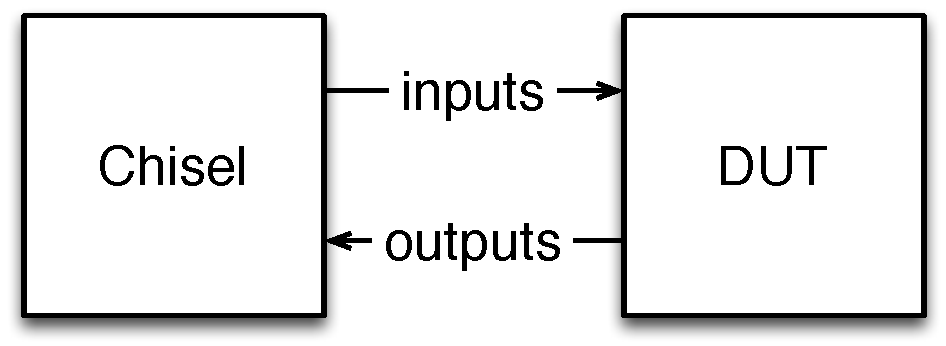
\includegraphics[width=0.45\textwidth]{../tutorial/figs/DUT.pdf}
\end{center}
\caption{DUT run using a Tester object in Scala with stdin and stdout connected}
\label{fig:dut}
\end{figure}
 
Testing is a crucial part of circuit design, 
and thus in Chisel we provide a mechanism for
testing circuits by providing test vectors within Scala using
subclasses of the \code{Tester} class:

\begin{scala}
class Tester[T <: Module] (val c: T, val isTrace: Boolean = true) {
  var t: Int
  var ok: Boolean
  val rnd: Random
  def int(x: Boolean): BigInt
  def int(x: Int): BigInt
  def int(x: Bits): BigInt
  def reset(n: Int = 1)
  def step(n: Int): Int
  def pokeAt(data: Mem[T], index: Int, x: BigInt)
  def poke(data: Bits, x: BigInt)
  def poke(data: Aggregate, x: Array[BigInt])
  def peekAt(data: Mem[T], index: Int)
  def peek(data: Bits): BigInt
  def peek(data: Aggregate): Array[BigInt]
  def expect (good: Boolean, msg: String): Boolean
  def expect (data: Bits, target: BigInt): Boolean
}
\end{scala}

\noindent
which binds a tester to a module
and allows users to write tests using the given debug protocol.  In particular, users utilize:
\begin{itemize}
\item \code{poke} to set input port and state values,
\item \code{step} to execute the circuit one time unit,
\item \code{peek} to read port and state values, and
\item \code{expect} to compare peeked circuit values to expected arguments.
\end{itemize}

\noindent
Users connect tester instances to modules using:


\begin{scala}
object chiselMainTest {
  def apply[T <: Module]
    (args: Array[String], comp: () => T)(
     tester: T => Tester[T]): T
}
\end{scala}

\noindent
When \code{-{-}test} is given as an argument to \code{chiselMainTest}, a
tester instance runs the Design Under Test (DUT) in a separate
process with \code{stdin} and \code{stdout} connected so that debug commands can 
be sent to the DUT and responses can be received from the DUT as shown in
Figure~\ref{fig:dut}.
\noindent

For example, in the following:

\begin{scala}
class Mux2Tests(c: Mux2) extends Tester(c) {
  val n = pow(2, 3).toInt
  for (s <- 0 until 2) {
    for (i0 <- 0 until 2) {
      for (i1 <- 0 until 2) {
        poke(c.io.sel, s)
        poke(c.io.in1, i1)
        poke(c.io.in0, i0)
        step(1)
        expect(c.io.out, (if (s == 1) i1 else i0))
      }
    }
  }
}
\end{scala}

\noindent
assignments for each input of \verb+Mux2+ is set to the appropriate values using \verb+poke+. For this particular example, we are testing the \verb+Mux2+ by hardcoding the inputs to some known values and checking if the output corresponds to the known one. To do this, on each iteration we generate appropriate inputs to the module and tell the simulation to assign these values to the inputs of the device we are testing \verb+c+, step the circuit, and test the expected value.  
\comment{Maybe elaborate a little bit what a step does. I assume it is one clock tick
Is a step needed as well for testing plain combinational circuits?}
Finally, the following shows how the tester is invoked:

\begin{scala}
chiselMainTest(args + "--test", () => Module(new Mux2())){ 
  c => new Mux2Tests(c) 
}
\end{scala}

Other command arguments are as follows:
\begin{tabular}{lll}
\verb+--targetDir+ & target pathname prefix \\
\verb+--genHarness+ & generate harness file for C++ \\
\verb+--backend v+ & generate verilog \\
\verb+--backend c+ & generate C++ (default)\\
\verb+--vcd+ & enable vcd dumping \\
\verb+--debug+ & put all wires in class file \\
\end{tabular}

\comment{What does it mean to generate a harness file?}

\section{State Elements}
\label{sec:sequential}

% SINGLE CLK and RESET

The simplest form of state element supported by Chisel is a
positive edge-triggered register, which can be instantiated
as:
\begin{scala}
val reg = Reg(next = in)
\end{scala}

\noindent
This circuit has an output that is a copy of the input signal \verb+in+
delayed by one clock cycle.  Note that we do not have to specify the
type of \verb+Reg+ as it will be automatically inferred from its input
when instantiated in this way.  In the current version of Chisel,
clock and reset are global signals that are implicity included where
needed.

Using registers, we can quickly define a number of useful circuit
constructs.  For example, a rising-edge detector that takes a boolean
signal in and outputs true when the current value is true and the
previous value is false is given by:
\begin{scala}
def risingedge(x: Bool) = x && !Reg(next = x)
\end{scala}

Counters are an important sequential circuit.  To construct an
up-counter that counts up to a maximum value, \verb+max+, then wraps
around back to zero (i.e., modulo \verb!max+1!), we write:
\begin{scala}
def counter(max: UInt) = {
  val x = Reg(init = UInt(0, max.getWidth))
  x := Mux(x === max, UInt(0), x + UInt(1))
  x
}
\end{scala}

\noindent
The counter register is created in the \verb!counter! function 
with a reset value of \verb!0! (with width large enough to hold \verb+max+),
to which the register will be initialized when the global reset for the circuit is asserted.
The \verb!:=! assignment to \verb!x! in \verb!counter! wires an update combinational circuit 
which increments the counter value unless it hits the \verb+max+ at which point it wraps back to zero.
Note that when \verb!x! appears on the right-hand side of
an assigment, its output is referenced, whereas when on the left-hand
side, its input is referenced.

Counters can be used to build a number of useful sequential circuits.
For example, we can build a pulse generator by outputting true when
a counter reaches zero:
\begin{scala}
// Produce pulse every n cycles.
def pulse(n: UInt) = counter(n - UInt(1)) === UInt(0)
\end{scala}

\noindent
A square-wave generator can then be toggled by the pulse train,
toggling between true and false on each pulse:
\begin{scala}[escapechar=@]
// Flip internal state when input true.
def toggle(p: Bool) = {
  val x = Reg(init = Bool(false))
  x := Mux(p, !x, x)
  x
}

// Square wave of a given period.
def squareWave(period: UInt) = toggle(pulse(period/2))
\end{scala}

\subsection{Forward Declarations}

Purely combinational circuits cannot have cycles between nodes, and
Chisel will report an error if such a cycle is detected.  Because they
do not have cycles, combinational circuits can always be constructed
in a feed-forward manner, by adding new nodes whose inputs are derived
from nodes that have already been defined.  Sequential circuits
naturally have feedback between nodes, and so it is sometimes
necessary to reference an output wire before the producing node has
been defined.  Because Scala evaluates program statements
sequentially, we allow data nodes to serve as a wire providing
a declaration of a node that can be used immediately, but whose
input will be set later.  
For example, in a simple CPU, we need to define the \verb!pcPlus4!
and \verb!brTarget! wires so they can be referenced before defined:
\begin{scala}
val pcPlus4  = UInt()
val brTarget = UInt()
val pcNext   = Mux(io.ctrl.pcSel, brTarget, pcPlus4)
val pcReg    = Reg(next = pcNext, init = UInt(0, 32))
pcPlus4     := pcReg + UInt(4)
...
brTarget    := addOut
\end{scala}

\noindent
The wiring operator
\verb!:=! is used to wire up
the connection after \verb!pcReg! and \verb!addOut! are defined.

\subsection{Conditional Updates}

In our previous examples using registers, we simply wired their inputs
to combinational logic blocks.  When describing the operation of state
elements, it is often useful to instead specify when updates to the
registers will occur and to specify these updates spread across
several separate statements.  Chisel provides conditional update rules
in the form of the \code{when} construct to support this style of
sequential logic description. For example,
\begin{scala}
val r = Reg(UInt(16))
when (c === UInt(0) ) {
  r := r + UInt(1)
}
\end{scala}

\noindent
where register \code{r} is updated at the end of the current clock
cycle only if \verb+c+ is zero.  The argument to \code{when} is a
predicate circuit expression that returns a \code{Bool}.  The update
block following \code{when} can only contain update statements using
the assignment operator \verb+:=+, simple expressions, and named wires
defined with \code{val}.

In a sequence of conditional updates, the last conditional update
whose condition is true takes priority.  For example,
\begin{scala}
when (c1) { r := UInt(1) }
when (c2) { r := UInt(2) }
\end{scala}

\noindent
leads to \code{r} being updated according to the following truth table:
\begin{center}
{\small
\begin{tabular}{|c|c|c|l|}
\hline
c1 & c2  &  r & \\
\hline
0 &  0 & r &  r unchanged \\
0 &  1 & 2 & \\
1 &  0 & 1 & \\
1 &  1 & 2& c2 takes precedence over c1 \\
\hline
\end{tabular}
}
\end{center}

\begin{figure}[h]
\centering
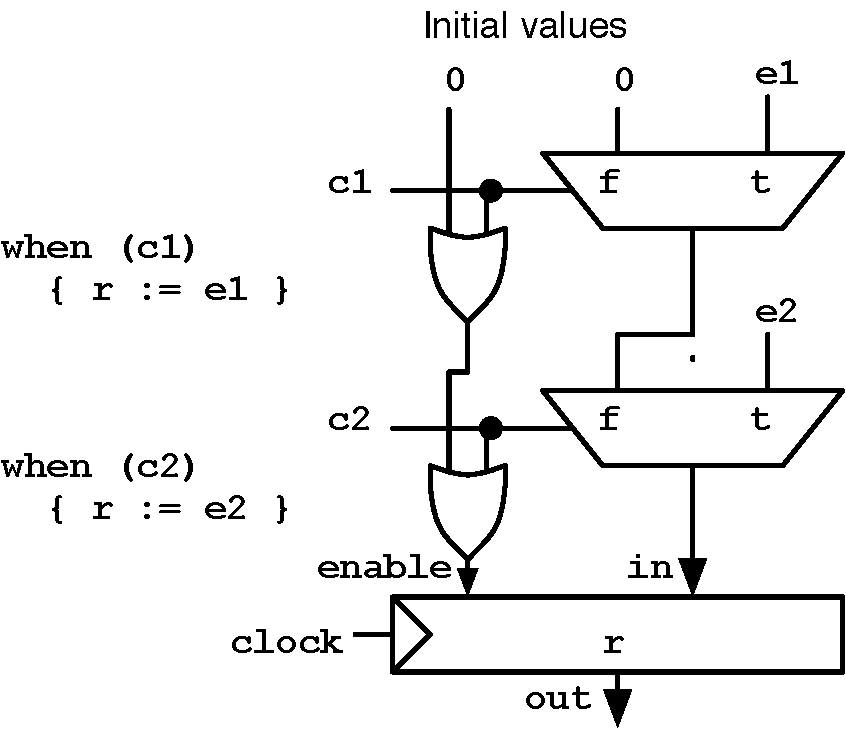
\includegraphics[width=3in]{figs/condupdates.pdf}
\caption{Equivalent hardware constructed for conditional updates.
  Each \code{when} statement adds another level of data mux and ORs
  the predicate into the enable chain.  The compiler effectively adds
  the termination values to the end of the chain automatically.}
\label{fig:condupdates}
\end{figure}

Figure~\ref{fig:condupdates} shows how each conditional update can be
viewed as inserting a mux before the input of a register to select
either the update expression or the previous input according to the
\code{when} predicate.  In addition, the predicate is OR-ed into a
firing signal that drives the load enable of the register.  The
compiler places initialization values at the beginning of the chain so
that if no conditional updates fire in a clock cycle, the load enable
of the register will be deasserted and the register value will not
change.
 
Chisel provides some syntactic sugar for other common forms of
conditional update.  The \verb+unless+ construct is the same as
\verb+when+ but negates its condition.  In other words,
\begin{scala}
unless (c) { body }
\end{scala}
is the same as
\begin{scala}
when (!c) { body }
\end{scala}

% The \verb+otherwise+ construct is the same as \verb+when+ with a true
% condition.  In other words,
% \begin{scala}
% otherwise { body }
% \end{scala}
% 
% \noindent
% is the same as
% \begin{scala}
% when (Bool(true)) { body }
% \end{scala}

The update block can target multiple registers, and there can be
different overlapping subsets of registers present in different update
blocks.  Each register is only affected by conditions in which it
appears.  The same is possible for combinational circuits (update
of a \code{Wire}). Note that all combinational
circuits need a default value. For example:
\begin{scala}
r := SInt(3); s := SInt(3)
when (c1)   { r := SInt(1); s := SInt(1) }
when (c2)   { r := SInt(2) }
\end{scala}

\noindent
leads to \code{r} and \code{s} being updated according to the
following truth table:
\begin{scala}
c1 c2  r  s
0   0  3  3
0   1  2  3 // r updated in c2 block, s at top level.
1   0  1  1
1   1  2  1
\end{scala}

\begin{commentary}
We are considering adding a different form of conditional update,
where only a single update block will take effect.  These atomic
updates are similar to Bluespec guarded atomic actions.
% TODO: when / .elsewhen / .otherwise
\end{commentary}

Conditional update constructs can be nested and any given block is
executed under the conjunction of all outer nesting conditions.  For
example,
\begin{scala}
when (a) { when (b) { body } }
\end{scala}

\noindent
is the same as:
\begin{scala}
when (a && b) { body }
\end{scala}

Conditionals can be chained together using
\verb+when+, \verb+.elsewhen+, \verb+.otherwise+ corresponding to
\verb+if+, \verb+else if+ and \verb+else+ in Scala.  For example,
\begin{scala}
when (c1) { u1 }
.elsewhen (c2) { u2 }
.otherwise { ud }
\end{scala}
\noindent
is the same as:
\begin{scala}
when (c1) { u1 }
when (!c1 && c2) { u2 }
when (!(c1 || c2)) { ud }
\end{scala}

We introduce the \code{switch} statement for conditional updates
involving a series of comparisons against a common key.  For example,
\begin{scala}
switch(idx) {
 is(v1) { u1 }
 is(v2) { u2 }
}
\end{scala}

\noindent
is equivalent to:
\begin{scala}
when (idx === v1) { u1 }
.elsewhen (idx === v2) { u2 }
\end{scala}

Chisel also allows a \code{Wire}, i.e., the output of some
combinational logic, to be the target of conditional update statements
to allow complex combinational logic expressions to be built
incrementally.  Chisel does not allow a combinational output to be
incompletely specified and will report an error if an unconditional
update is not encountered for a combinational output.
\begin{commentary}
In Verilog, if a procedural specification of a combinational logic
block is incomplete, a latch will silently be inferred causing many
frustrating bugs.

It could be possible to add more analysis to the Chisel compiler, to
determine if a set of predicates covers all possibilities.  But for
now, we require a single predicate that is always true in the
chain of conditional updates to a \code{Wire}.
\end{commentary}


\subsection{Finite State Machines}

A common type of sequential circuit used in digital design is a Finite
State Machine (FSM).  An example of a simple FSM is a parity
generator:

% \begin{scala}
% class Parity extends Module {
%   val io = new Bundle {
%     val in  = Bool(INPUT)
%     val out = Bool(OUTPUT) }
%   val s_even :: s_odd :: Nil = Enum(2, UInt())
%   val state  = Reg(init = s_even)
%   switch(state, Array(
%     (s_even, () => { when (io.in) { state := s_odd } }),
%     (s_odd,  () => { when (io.in) { state := s_even } }) ))
%   io.out := state === s_odd
% }
% \end{scala}

\begin{scala}
class Parity extends Module {
  val io = new Bundle {
    val in  = Bool(dir = INPUT)
    val out = Bool(dir = OUTPUT) }
  val s_even :: s_odd :: Nil = Enum(UInt(), 2)
  val state  = Reg(init = s_even)
  when (io.in) {
    when (state === s_even) { state := s_odd  }
    when (state === s_odd)  { state := s_even }
  }
  io.out := (state === s_odd)
}
\end{scala}

\noindent
where \verb+Enum(UInt(), 2)+ generates two \verb+UInt+ literals and
where the states are updated when \verb+in+ is true.  It is worth
noting that all of the mechanisms for FSMs are built upon registers,
wires, and conditional updates.

Below is a more complicated FSM example which is a circuit for
accepting money for a vending machine:
\begin{scala}
class VendingMachine extends Module {
  val io = new Bundle {
    val nickel = Bool(dir = INPUT)
    val dime   = Bool(dir = INPUT)
    val valid    = Bool(dir = OUTPUT) }
  val s_idle :: s_5 :: s_10 :: s_15 :: s_ok :: Nil = 
    Enum(UInt(), 5)
  val state = Reg(init = s_idle)
  when (state === s_idle) {
    when (io.nickel) { state := s_5 }
    when (io.dime)   { state := s_10 }
  }
  when (state === s_5) {
    when (io.nickel) { state := s_10 }
    when (io.dime)   { state := s_15 }
  }
  when (state === s_10) {
    when (io.nickel) { state := s_15 }
    when (io.dime)   { state := s_ok }
  }
  when (state === s_15) {
    when (io.nickel) { state := s_ok }
    when (io.dime)   { state := s_ok }
  }
  when (state === s_ok) {
    state := s_idle
  }
  io.valid := (state === s_ok)
}
\end{scala}

\noindent
Here is the vending machine FSM defined with \code{switch} statement:
\begin{scala}
class VendingMachine extends Module {
  val io = new Bundle {
    val nickel = Bool(dir = INPUT)
    val dime   = Bool(dir = INPUT)
    val valid    = Bool(dir = OUTPUT)
  }
  val s_idle :: s_5 :: s_10 :: s_15 :: s_ok :: Nil = Enum(UInt(), 5)
  val state = Reg(init = s_idle)
  
  switch (state) {
    is (s_idle) {
      when (io.nickel) { state := s_5 }
      when (io.dime) { state := s_10 }
    }
    is (s_5) {
      when (io.nickel) { state := s_10 }
      when (io.dime) { state := s_15 }
    }
    is (s_10) {
      when (io.nickel) { state := s_15 }
      when (io.dime) { state := s_ok }
    }
    is (s_15) {
      when (io.nickel) { state := s_ok }
      when (io.dime) { state := s_ok }
    }
    is (s_ok) {
      state := s_idle
    }
  }
  io.valid := (state ===s_ok)
}
\end{scala}

\section{Memories}

Chisel provides facilities for creating both read only and
read/write memories.  

\subsection{ROM}

Users can define read only memories with a \code{Vec}:

\begin{scala}
Vec(inits: Seq[T])
Vec(elt0: T, elts: T*)
\end{scala}

\noindent
where \verb+inits+ is a sequence of initial \verb+Data+ literals that
initialize the ROM.
For example,  users can
create a small ROM initialized to \verb+1, 2, 4, 8+ and 
loop through all values using a counter as an address generator as follows:

\begin{scala}
val m = Vec(Array(UInt(1), UInt(2), UInt(4), UInt(8)))
val r = m(counter(UInt(m.length)))
\end{scala}

\noindent
We can create an \verb+n+ value sine lookup table using a ROM initialized as follows:

\begin{scala}
def sinTable (amp: Double, n: Int) = {
  val times = 
    Range(0, n, 1).map(i => (i*2*Pi)/(n.toDouble-1) - Pi)
  val inits = 
    times.map(t => SInt(round(amp * sin(t)), width = 32))
  Vec(inits)
}
def sinWave (amp: Double, n: Int) = 
  sinTable(amp, n)(counter(UInt(n))
\end{scala}

\noindent
where \verb+amp+ is used to scale the fixpoint values stored in the ROM.

\subsection{Mem}

Memories are given special treatment in Chisel since hardware
implementations of memory have many variations, e.g., FPGA memories
are instantiated quite differently from ASIC memories.  Chisel defines
a memory abstraction that can map to either simple Verilog behavioral
descriptions, or to instances of memory modules that are available
from external memory generators provided by foundry or IP vendors.  

Chisel supports random-access memories via the \code{Mem} construct.
Writes to Mems are positive-edge-triggered and reads are either
combinational or positive-edge-triggered.

\begin{scala}
object Mem {
  def apply[T <: Data](type: T, depth: Int, 
          seqRead: Boolean = false): Mem
}

class Mem[T <: Data](type: T, depth: Int,
      seqRead: Boolean = false)
    extends Updateable {
  def apply(idx: UInt): T
}
\end{scala}

Ports into Mems are created by applying a \code{UInt} index.  A 32-entry
register file with one write port and two combinational read ports might be
expressed as follows:

\begin{scala}
val rf = Mem(UInt(width = 64), 32)
when (wen) { rf(waddr) := wdata }
val dout1 = rf(waddr1)
val dout2 = rf(waddr2)
\end{scala}

If the optional parameter \code{seqRead} is set, Chisel will attempt to infer
sequential read ports when the read address is a Reg.  A one-read,
one-write SRAM might be described as follows:

\begin{scala}
val ram1r1w =
  Mem(UInt(width = 32), 1024, seqRead = true)
val reg_raddr = Reg(UInt())
when (wen) { ram1r1w(waddr) := wdata }
when (ren) { reg_raddr := raddr }
val rdata = ram1r1w(reg_raddr)
\end{scala}

Single-ported SRAMs can be inferred when the read and write conditions are
mutually exclusive in the same \code{when} chain:

\begin{scala}
val ram1p = 
  Mem(UInt(width = 32), 1024, seqRead = true)
val reg_raddr = Reg(UInt())
when (wen) { ram1p(waddr) := wdata }
.elsewhen (ren) { reg_raddr := raddr }
val rdata = ram1p(reg_raddr)
\end{scala}

If the same Mem address is both written and sequentially read on the same clock
edge, or if a sequential read enable is cleared, then the read data is
undefined.

Mem also supports write masks for subword writes.  A given bit is written if
the corresponding mask bit is set.

\begin{scala}
val ram = Mem(UInt(width = 32), 256)
when (wen) { ram.write(waddr, wdata, wmask) }
\end{scala}


% For example, an
% audio recorder could be defined as follows:
% 
% \begin{scala}
%   def audioRecorder(n: Int, button: Bool) = { 
%     val addr   = counter(UInt(n))
%     val ram    = Mem(n)
%     ram(addr) := button
%     ram(Mux(button(), UInt(0), addr))
%   } 
% \end{scala}
% 
% \noindent
% where a counter is used as an address generator into a memory.  
% The device records while \verb+button+ is \verb+true+, or plays back when \verb+false+.


\section{Interfaces and Bulk Connections}
\label{sec:interfaces}

For more sophisticated modules it is often useful to define and
instantiate interface classes while defining module IO.  First and
foremost, interface classes promote reuse allowing users to capture
once and for all common interfaces in a useful form.  Secondly,
interfaces allow users to dramatically reduce wiring by supporting
{\em bulk connections} between producer and consumer modules.  Finally,
users can make changes in large interfaces in one place reducing the
number of updates required when adding or removing pieces of the
interface.

\subsection{Port Classes, Subclasses, and Nesting}

As we saw earlier, users can define their own interfaces by defining a class that subclasses \verb+Bundle+.  
For example, a user could define a simple link for handshaking data as follows:

\begin{scala}
class SimpleLink extends Bundle { 
  val data  = UInt(16, OUTPUT) 
  val valid = Bool(OUTPUT)
}
\end{scala}

\noindent
We can then extend \verb+SimpleLink+ by adding parity bits using
bundle inheritance:

\begin{scala}
class PLink extends SimpleLink { 
  val parity = UInt(5, OUTPUT) 
}
\end{scala}

\noindent
In general, users can organize their interfaces into hierarchies using inheritance.  

From there we can define a filter interface by nesting two
\verb+PLink+s into a new \verb+FilterIO+ bundle:

\begin{scala}
class FilterIO extends Bundle { 
  val x = new PLink().flip
  val y = new PLink()
}
\end{scala}

\noindent
where \verb+flip+ recursively changes the ``gender'' of a bundle,
changing input to output and output to input.

We can now define a filter by defining a filter class extending module:

\begin{scala}
class Filter extends Module { 
  val io = new FilterIO()
  ...
}
\end{scala}

\noindent 
where the \verb+io+ field contains \verb+FilterIO+. 

\subsection{Bundle Vectors}

Beyond single elements, vectors of elements form richer hierarchical interfaces.  
For example, in order to create a crossbar with a vector of inputs, producing a vector of outputs, and selected by a UInt input, 
we utilize the \verb+Vec+ constructor:

\begin{scala}
class CrossbarIo(n: Int) extends Bundle {
  val in  = Vec.fill(n){ new PLink().flip() }
  val sel = UInt(INPUT, sizeof(n))
  val out = Vec.fill(n){ new PLink() }
}
\end{scala}

% \begin{scala}
% class CrossbarIo(n: Int) extends Bundle {
%   val in  = Vec.fill(n){ UInt(w, INPUT) }
%   val sel = Vec.fill(n){ UInt(sizeof(n),  INPUT) }
%   val out = Vec.fill(n){ UInt(w, OUTPUT) }
% }
% \end{scala}

\noindent
where \verb+Vec+ takes a size as the first argument and a block returning a port as the second argument.

\subsection{Bulk Connections}

We can now compose two filters into a filter block as follows:

\begin{scala}
class Block extends Module { 
  val io = new FilterIO()
  val f1 = Module(new Filter())
  val f2 = Module(new Filter())

  f1.io.x <> io.x
  f1.io.y <> f2.io.x
  f2.io.y <> io.y
}
\end{scala}

\noindent
where \verb+<>+ bulk connects interfaces of opposite gender between
sibling modules or interfaces of same gender between parent/child modules. 
Bulk connections connect leaf ports of the same name to each other.
After all connections are made and the circuit is being elaborated,
Chisel warns users if ports have other than exactly one connection to them.

\subsection{Interface Views}

\begin{figure}
\centerline{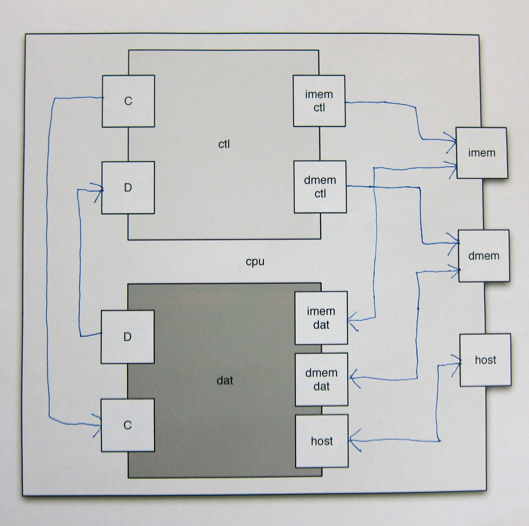
\includegraphics[width=3in]{figs/cpu.png}}
\caption{Simple CPU involving control and data path submodules and host and memory interfaces.}
\label{fig:cpu}
\end{figure}

Consider a simple CPU consisting of control path and data path submodules and host and memory interfaces shown in Figure~\ref{fig:cpu}.
In this CPU we can see that the control path and data path each connect only to a part of the instruction and data memory interfaces. 
Chisel allows users to do this with partial fulfillment of interfaces.
A user first defines the complete interface to a ROM and Mem as follows:

\begin{scala}
class RomIo extends Bundle {
  val isVal = Bool(INPUT)
  val raddr = UInt(INPUT, 32)
  val rdata = UInt(OUTPUT, 32)
}

class RamIo extends RomIo {
  val isWr  = Bool(INPUT)
  val wdata = UInt(INPUT, 32)
}
\end{scala}

\noindent
Now the control path can build an interface in terms of these interfaces:

\begin{scala}
class CpathIo extends Bundle {
  val imem = RomIo().flip()
  val dmem = RamIo().flip()
  ...
}
\end{scala}

\noindent
and the control and data path modules can be built by partially assigning to
this interfaces as follows:

\begin{scala}
class Cpath extends Module {
  val io = new CpathIo();
  ...
  io.imem.isVal := ...;
  io.dmem.isVal := ...;
  io.dmem.isWr  := ...;
  ...
}

class Dpath extends Module {
  val io = new DpathIo();
  ...
  io.imem.raddr := ...;
  io.dmem.raddr := ...;
  io.dmem.wdata := ...;
  ...
}
\end{scala}

\noindent
We can now wire up the CPU using bulk connects as we would with other bundles:

\begin{scala}
class Cpu extends Module {
  val io = new CpuIo()
  val c  = Module(new CtlPath())
  val d  = Module(new DatPath())
  c.io.ctl  <> d.io.ctl
  c.io.dat  <> d.io.dat
  c.io.imem <> io.imem
  d.io.imem <> io.imem
  c.io.dmem <> io.dmem
  d.io.dmem <> io.dmem
  d.io.host <> io.host
}
\end{scala}

\noindent
Repeated bulk connections of partially assigned control and data path interfaces
completely connect up the CPU interface.

% A Bool can be automatically treated as a single bit UInt (with values
% 0 or 1), but an Int or UInt cannot be used as a Bool without an
% explicit cast.
%
%   Lit(5) // means a constant node with decimal value 5. Bit width will
%           // be inferred automatically if possible
%
% A node is a hardware operator that has zero or more inputs and that
% drives one output.  An example of a node with zero inputs is a
% constant generator.
%
% \begin{scala}
% Lit(10, 4) // means a constant node of type UInt that is 4 bits
%            // wide with decimal 10.
% Lit(10)
% LitInt(10, 4)
% LitUInt(10, 4)
% Lit(-1,4)
% \end{scala}
%
% can more concisely write:
%
% Module correspond to Verilog modules
% Cell is a sub-module, Chisel Module

\section{Functional Creation of Modules}
\label{sec:funconstructor}

It is also useful to be able to make a functional interface for
module construction.  For instance, we could build a constructor
that takes multiplexer inputs as parameters and returns the
multiplexer output:

\begin{scala}
object Mux2 {
  def apply (sel: UInt, in0: UInt, in1: UInt) = {
    val m = new Mux2()
    m.io.in0 := in0
    m.io.in1 := in1
    m.io.sel := sel
    m.io.out
  }
}
\end{scala}

\noindent
where \code{object Mux2} creates a Scala singleton object on the \code{Mux2}
module class, and \code{apply} defines a method for creation of a \code{Mux2} instance.
%
With this \code{Mux2} creation function, the specification of \code{Mux4} now is
significantly simpler.

\begin{scala}
class Mux4 extends Module {
  val io = new Bundle {
    val in0 = UInt(INPUT, 1)
    val in1 = UInt(INPUT, 1)
    val in2 = UInt(INPUT, 1)
    val in3 = UInt(INPUT, 1)
    val sel = UInt(INPUT, 2)
    val out = UInt(OUTPUT, 1)
  }
  io.out := Mux2(io.sel(1),
                 Mux2(io.sel(0), io.in0, io.in1),
                 Mux2(io.sel(0), io.in2, io.in3))
}
\end{scala}

Selecting inputs is so useful that Chisel builds it in and calls it
\code{Mux}.  However, unlike \code{Mux2} defined above, the builtin version allows any datatype on
\code{in0} and \code{in1} as long as they have a common super class.
In Section~\ref{sec:parameterization} we will see how to define this
ourselves.

Chisel provides \code{MuxCase} which is an n-way \code{Mux} 
\begin{scala}
MuxCase(default, Array(c1 -> a, c2 -> b, ...))
\end{scala}
 
\noindent
where each condition / value is represented as a tuple in a Scala
array and where \code{MuxCase} can be translated into the following
\code{Mux} expression:

\begin{scala}
Mux(c1, a, Mux(c2, b, Mux(..., default)))
\end{scala}

\noindent
Chisel also provides \code{MuxLookup} which is an n-way indexed multiplexer:

\begin{scala}
MuxLookup(idx, default, 
          Array(UInt(0) -> a, UInt(1) -> b, ...))
\end{scala}

\noindent
which can be rewritten in terms of:\verb+MuxCase+ as follows:

\begin{scala}
MuxCase(default, 
        Array((idx === UInt(0)) -> a, 
              (idx === UInt(1)) -> b, ...))
\end{scala}

\noindent
Note that the cases (eg. c1, c2) must be in parentheses.

% TODO: higher order filter

% \Noindent
% where the overall expression returns the value corresponding to the first condition evaluating to true.

% FUNCTIONAL CREATION
%
% want to go from io to constructor
%
% \begin{scala}
% val io = new Bundle{
%   val sel = UInt(INPUT, 1)
%   val in0 = UInt(INPUT, 1)
%   val in1 = UInt(INPUT, 1)
%   val out = UInt(OUTPUT, 1)
% }
% def Mux2(sel: UInt, in0: UInt, in0: UInt): UInt = {
%   val m = new Mux2()
%   m.io.wire(Array("sel" => sel, "in0" => in0, "in1" => in1), "out")
% }
% \end{scala}

% picture of box in box



%%%%%%%%%%%%%%%%%%%%%%%%%%%%%%%%%%%%%%%%%%%%%%%%%%%%%%%%%%%%%%%%%%%%%%%%%%%%%%%%%%%%%%%%%%%%%%%%%%%%%%%%%%%%%%
\section{Polymorphism and Parameterization}
\label{sec:parameterization}

Scala is a strongly typed language and uses parameterized types to specify generic functions and classes.  
In this section, we show how Chisel users can define their own reusable functions and classes using parameterized classes.
\begin{commentary}
This section is advanced and can be skipped at first reading.
\end{commentary}

\subsection{Parameterized Functions}

Earlier we defined \code{Mux2} on \code{Bool}, but now we show how we can define a generic multiplexer function.
We define this function as taking a boolean condition and con and alt arguments (corresponding to then and else expressions) of type \code{T}:

\begin{scala}
def Mux[T <: Bits](c: Bool, con: T, alt: T): T { ... }
\end{scala}

\noindent
where \code{T} is required to be a subclass of \code{Bits}.
Scala ensures that in each usage of \code{Mux}, it can find a common superclass of the actual con and alt argument types, 
otherwise it causes a Scala compilation type error.
For example,

\begin{scala}
Mux(c, UInt(10), UInt(11))
\end{scala}

\noindent
yields a \code{UInt} wire because the \code{con} and \code{alt} arguments are each of type \code{UInt}.

% Earlier we defined \code{Mux2} on \code{Bool}, but now we show how we can define a generic \code{Mux}.  
% We define a function that takes a condition and two functions of no arguments (called thunks) for the {\it then} and {\it else} cases:
% 
% \begin{scala}
% def Mux[T <: UInt](c: Bool, con: T, alt: T): T
% def Mux[T <: UInt](c: Bool)(con: => T)(alt: => T): T
% \end{scala}
% 
% \noindent
% where the two thunk return types are parameterized to be a type \code{T} that is a subclass of \code{UInt}.
% Scala ensures that it finds a common superclass of the two thunks' return types.

We now present a more advanced example of parameterized functions for defining an inner product FIR digital filter generically over Chisel \code{Num}'s.
The inner product FIR filter can be mathematically defined as:
\begin{equation}
y[t] = \sum_j w_j * x_j[t-j]
\end{equation}

\noindent 
where $x$ is the input and $w$ is a vector of weights.
In Chisel this can be defined as:

% MS: just out of curiosity: does this example generate several delay lines?
\begin{scala}
def delays[T <: Data](x: T, n: Int): List[T] = 
  if (n <= 1) List(x) else x :: Delays(RegNext(x), n-1)

def FIR[T <: Data with Num[T]](ws: Seq[T], x: T): T = 
  (ws, Delays(x, ws.length)).zipped.
    map( _ * _ ).reduce( _ + _ )
\end{scala}
 
\noindent
where 
\code{delays} creates a list of incrementally increasing delays of its input and
\code{reduce} constructs a reduction circuit given a binary combiner function \code{f}.  
In this case, \code{reduce} creates a summation circuit.
Finally, the \code{FIR} function is constrained to work on inputs of type \code{Num} where Chisel multiplication and addition are defined.

\subsection{Parameterized Classes}

Like parameterized functions, we can also parameterize classes to make them more reusable.
For instance, we can generalize the Filter class to use any kind of link.  
We do so by parameterizing the \verb+FilterIO+ class and defining the constructor to take a zero argument type constructor function as follow:

\begin{scala}
class FilterIO[T <: Data](type: T) extends Bundle { 
  val x = type.asInput.flip
  val y = type.asOutput
}
\end{scala}

\noindent
We can now define \verb+Filter+ by defining a module class that also takes a link type constructor argument and passes it through to the \verb+FilterIO+ interface constructor:

\begin{scala}
class Filter[T <: Data](type: T) extends Module { 
  val io = new FilterIO(type)
  ...
}
\end{scala}

\noindent
We can now define a \verb+PLink+ based \verb+Filter+ as follows:
\begin{scala}
val f = Module(new Filter(new PLink()))
\end{scala}

\noindent
where the curly braces \verb+{ }+ denote a zero argument function (aka thunk) that in this case creates the link type.

A generic FIFO could be defined as shown in Figure~\ref{fig:fifo} and
used as follows:

\begin{scala}
class DataBundle extends Bundle {
  val A = UInt(width = 32)
  val B = UInt(width = 32)
}

object FifoDemo {
  def apply () = new Fifo(new DataBundle, 32)
}
\end{scala}

\begin{figure}[ht]
\begin{scala}
class Fifo[T <: Data] (type: T, n: Int) 
    extends Module {
  val io = new Bundle {
    val enq_val = Bool(INPUT)
    val enq_rdy = Bool(OUTPUT)
    val deq_val = Bool(OUTPUT)
    val deq_rdy = Bool(INPUT)
    val enq_dat = type.asInput
    val deq_dat = type.asOutput
  }
  val enq_ptr      = Reg(init = UInt(0, sizeof(n)))
  val deq_ptr      = Reg(init = UInt(0, sizeof(n)))
  val is_full      = Reg(init = Bool(false))
  val do_enq       = io.enq_rdy && io.enq_val
  val do_deq       = io.deq_rdy && io.deq_val
  val is_empty     = !is_full && (enq_ptr === deq_ptr)
  val deq_ptr_inc  = deq_ptr + UInt(1)
  val enq_ptr_inc  = enq_ptr + UInt(1)
  val is_full_next = 
    Mux(do_enq && ~do_deq && (enq_ptr_inc === deq_ptr), 
        Bool(true),
        Mux(do_deq && is_full, Bool(false), is_full))
  enq_ptr := Mux(do_enq, enq_ptr_inc, enq_ptr)
  deq_ptr := Mux(do_deq, deq_ptr_inc, deq_ptr)
  is_full := is_full_next
  val ram = Mem(n)
  when (do_enq) {
    ram(enq_ptr) := io.enq_dat
  }
  io.enq_rdy := !is_full
  io.deq_val := !is_empty
  ram(deq_ptr) <> io.deq_dat
}
\end{scala}
\caption{Parameterized FIFO example.}
\label{fig:fifo}
\end{figure}

It is also possible to define a generic decoupled interface:

\begin{scala}
class DecoupledIO[T <: Data](data: T) 
    extends Bundle {
  val ready = Bool(INPUT)
  val valid = Bool(OUTPUT)
  val bits  = data.clone.asOutput
}
\end{scala}

\noindent
This template can then be used to add a handshaking protocol to any
set of signals:

\begin{scala}
class DecoupledDemo 
  extends DecoupledIO()( new DataBundle )
\end{scala}

\noindent
The FIFO interface in Figure~\ref{fig:fifo} can be now be simplified as
follows: 

\begin{scala}
class Fifo[T <: Data] (data: T, n: Int) 
    extends Module {
  val io = new Bundle {
    val enq = new DecoupledIO( data ).flip()
    val deq = new DecoupledIO( data )
  }
  ...
}
\end{scala}


\section{Multiple Clock Domains}

Chisel 2.0 introduces support of multiple clock domains.  

\subsection{Creating Clock domains}

In order to use multiple clock domains, users must create multiple clocks.  
In Chisel, clocks are first class nodes created with a reset signal parameter and defined as follows:

\begin{scala}
class Clock (reset: Bool) extends Node {
  def reset: Bool // returns reset pin
}
\end{scala}

\noindent
% Having reset in clock makes it easier to pass around.
In Chisel there is a builtin implicit clock that state elements use by default:

\begin{scala}
var implicitClock = new Clock( implicitReset )
\end{scala}

The clock for state elements and modules can be defined using an additional named parameter called clock:

\begin{scala}
Reg(... clock: Clock = implicitClock)
Mem(... clock: Clock = implicitClock)
Module(... clock: Clock = implicitClock)
\end{scala}

\subsection{Crossing Clock Domains}

There are two ways that circuits can be defined to send data between clock domains.
The first and most primitive way is by using a synchronizer circuit comprised of two registers as follows:

\begin{scala}
// signalA is in clock domain clockA, 
// want a version in clockB as signalB
val s1 = Reg(init = UInt(0), clock = clockB)
val s2 = Reg(init = UInt(0), clock = clockB)
s1      := signalA
s2      := s1; 
signalB := s2
\end{scala}

\noindent
Due to metastability issues, this technique is limited to communicating one bit data between domains.

The second and more general way to send data between domains is by using an asynchronous queue:

\begin{scala}
class AsyncQueue[T<:Data]
    (gen: T, depth: Int, enq_clk: Clock, deq_clock: Clock)
  extends Module
\end{scala}

\noindent
When get a version of signalA from clock domains clockA to clockB by specifying the standard queue parameters and the two clocks and then using the standard decoupled ready/valid signals:

\begin{scala}
val queue = 
  new AsyncQueue(Uint(width = 32), 2, clockA, clockB)
fifo.enq.bits := signalA
signalB       := fifo.deq.bits
fifo.valid    := condA
fifo.ready    := condB
...
\end{scala}

\subsection{Backend Specific Multiple Clock Domains}

Each Chisel backend requires the user to setup up and control multiple clocks in a backend specific manner.  For the purposes of showing how to drive a multi clock design, consider the example of hardware with two modules communicating using an AsyncQueue with each module on separate clocks: \verb+fastClock+ and \verb+slowClock+.  

\subsubsection{C++}

In the C++ backend, for every clock \verb+i+ there is a
\begin{itemize}
\item \verb+uint64_t clk_i+ field representing the clock \verb+i+'s period,
\item \verb+uint63_t clk_i_cnt+ field representing the clock \verb+i+'s current count,
\item \verb+clock_lo_i+ and \verb+clock_hi_i+, 
\item \verb+int reset()+ function which ensures that all \verb+clock_lo+ and \verb+clock_hi+ functions are called at least once, and
\item \verb+int clock(reset)+ function which computes min delta, invokes appropriate \verb+clock_lo+ and \verb+clock_hi+'s and returns min delta used.
\end{itemize}

\noindent
In order to set up a C++ simulation, the user 
\begin{itemize}
\item initializes all period fields to desired period
\item initializes all count fields to desired phase, 
\item calls \verb+reset+ and then
\item repeated calls clock to step the simulation.
\end{itemize}

\noindent
The following is a C++ example of a main function for the \verb+slowClock+ / \verb+fastClock+ example:

\begin{scala}
int main(int argc, char** argv) {
  ClkDomainTest_t dut;
  dut.init(1);
  dut.clk = 2;
  dut.clk_cnt = 1;
  dut.fastClock = 4;
  dut.fastClock_cnt = 0;
  dut.slowClock = 6;
  dut.slowClock_cnt = 0;
  for (int i = 0; i < 12; i ++) 
    dut.reset();
  for (int i = 0; i < 96; i ++) 
    dut.clock(LIT<1>(0));
}
\end{scala}

\subsubsection{Verilog}

In Verilog, 

\begin{itemize}
\item Chisel creates a new port for each clock / reset,
\item Chisel wires all the clocks to the top module, and
\item the user must create an \verb+always+ block clock driver for every clock \verb+i+.
\end{itemize}

\noindent
The following is a Verilog example of a top level harness to drive the  \verb+slowClock+ / \verb+fastClock+ example circuit:

\begin{scala}
module emulator;
  reg fastClock = 0, slowClock = 0, 
      resetFast = 1, resetSlow = 1;
  wire [31:0] add, mul, test;
  always #2 fastClock = ~fastClock;
  always #4 slowClock = ~slowClock;
  initial begin
     #8 
     resetFast = 0;
     resetSlow = 0;
     #400
     $finish;
  end
  ClkDomainTest dut (
     .fastClock(fastClock),
     .slowClock(slowClock),
     .io_resetFast(resetFast),
     .io_resetSlow(resetSlow),
     .io_add(add), .io_mul(mul), .io_test(test));
endmodule
\end{scala}

\noindent
See \url{http://www.asic-world.com/verilog/verifaq2.html} for more information about simulating clocks in Verilog.

\section{Acknowlegements}

Many people have helped out in the design of Chisel, and we thank them
for their patience, bravery, and belief in a better way.  Many
Berkeley EECS students in the Isis group gave weekly feedback as the
design evolved including but not limited to Yunsup Lee, Andrew
Waterman, Scott Beamer, Chris Celio, etc.  Yunsup Lee gave us feedback
in response to the first RISC-V implementation, called TrainWreck,
translated from Verilog to Chisel.  Andrew Waterman and Yunsup Lee
helped us get our Verilog backend up and running and Chisel TrainWreck
running on an FPGA.  Brian Richards was the first actual Chisel user,
first translating (with Huy Vo) John Hauser's FPU Verilog code to
Chisel, and later implementing generic memory blocks.  Brian gave many
invaluable comments on the design and brought a vast experience in
hardware design and design tools.  Chris Batten shared his fast
multiword C++ template library that inspired our fast emulation
library.  Huy Vo became our undergraduate research assistant and was
the first to actually assist in the Chisel implementation.  We
appreciate all the EECS students who participated in the Chisel
bootcamp and proposed and worked on hardware design projects all of
which pushed the Chisel envelope.  We appreciate the work that James
Martin and Alex Williams did in writing and translating network and
memory controllers and non-blocking caches.  Finally, Chisel's
functional programming and bit-width inference ideas were inspired by
earlier work on a hardware description language called Gel~\cite{gel} designed in
collaboration with Dany Qumsiyeh and Mark Tobenkin.

% \note{Who else?}

\begin{thebibliography}{50}
\bibitem{chisel-dac12} Bachrach, J., Vo, H., Richards, B., Lee, Y., Waterman,
  A., Avi\v{z}ienis, Wawrzynek, J., Asanovi\'{c} \textsl{Chisel:
    Constructing Hardware in a Scala Embedded Language}.
in DAC '12.
\bibitem{gel} Bachrach, J., Qumsiyeh, D., Tobenkin, M. \textsl{Hardware Scripting in Gel}.
in Field-Programmable Custom Computing Machines, 2008. FCCM '08. 16th.
\end{thebibliography}

\end{document}
